\clearpage
\begin{examplebox}
\textbf{例1（典型即用：求定值）。}

双曲线 $\dfrac{x^2}{9}-\dfrac{y^2}{4}=1$ 上任取一点 $P$，
过 $P$ 分别作与两渐近线平行的直线，求所得平行四边形面积。

\textbf{解：} $a=3,b=2$，故
\[
\boxed{S=\frac{ab}{2}=3}.
\]
\textbf{即时自检：}取顶点 $P=(3,0)$，
$Q=(3/2,1)$、$R=(3/2,-1)$；
$S=|\det(Q,R)|=3$。
\end{examplebox}

\clearpage
\begin{examplebox}
\textbf{例2（点不在顶点：坐标验算）。}

仍取 $a=3,b=2$，令
\[
P=\left(\frac{13}{4},\frac56\right).
\]
图中 $k=2/3$，$(X,Y)$ 为直线上的动点坐标。
\begin{center}
% k=2/3 and P=(13/4,5/6); the labels give the general equations.
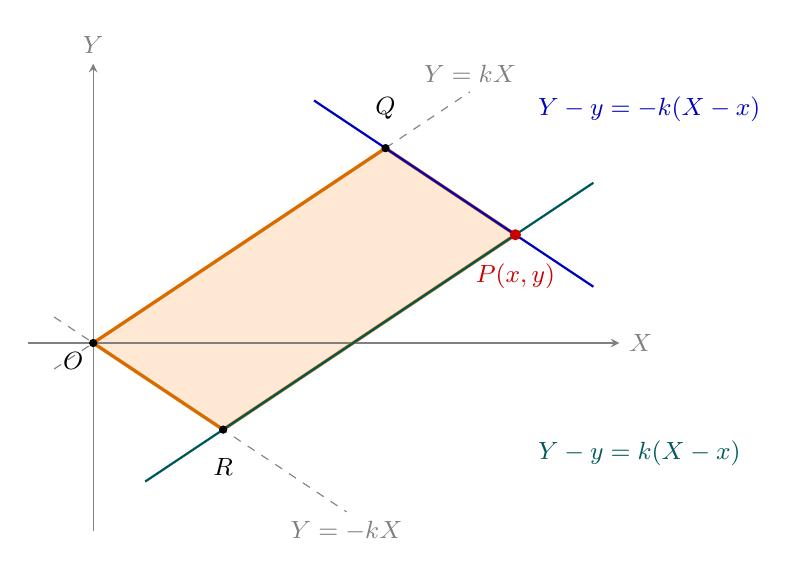
\begin{tikzpicture}[x=1.65cm,y=1.65cm,>=stealth,font=\small]
\coordinate (O) at (0,0); \coordinate (Q) at (2.25,1.5);
\coordinate (R) at (1,-2/3); \coordinate (P) at (3.25,5/6);
\fill[orange!17] (O)--(Q)--(P)--(R)--cycle;
\draw[->,gray] (-.5,0)--(4.05,0) node[right] {$X$};
\draw[->,gray] (0,-1.45)--(0,2.15) node[above] {$Y$};
\draw[gray,dashed] (-.3,-.2)--(2.9,29/15) node[above] {$Y=kX$};
\draw[gray,dashed] (-.3,.2)--(1.95,-1.3) node[below] {$Y=-kX$};
\draw[orange!85!black,very thick] (O)--(Q)--(P)--(R)--cycle;
\draw[blue!75!black,thick] (1.7,28/15)--(3.85,13/30);
\draw[teal!70!black,thick] (.4,-16/15)--(3.85,37/30);
\node[anchor=west,blue!75!black] at (3.35,1.8) {$Y-y=-k(X-x)$};
\node[anchor=west,teal!70!black] at (3.35,-.85) {$Y-y=k(X-x)$};
\fill (O) circle(1.5pt) node[below left] {$O$};
\fill (Q) circle(1.5pt) node[above=7pt] {$Q$};
\fill (R) circle(1.5pt) node[below=7pt] {$R$};
\fill[red!80!black] (P) circle(2pt) node[below=7pt] {$P(x,y)$};
\end{tikzpicture}

\end{center}
核对
\[
\frac{(13/4)^2}{9}-\frac{(5/6)^2}{4}
=\frac{169}{144}-\frac{25}{144}=1,
\]
故 $P\in H$。由交点公式
\[
Q=\left(\frac94,\frac32\right),\quad
R=\left(1,-\frac23\right).
\]
于是
\[
\boxed{S=\left|\frac94\cdot\left(-\frac23\right)
-\frac32\cdot1\right|=3}.
\]
\textbf{迁移信号：}点坐标看上去复杂，别先求交点；如果只问面积，\textbf{直接代 $ab/2$}。
\end{examplebox}

\clearpage
\begin{examplebox}
\textbf{例3（反求参数：已知面积定值）。}

若某双曲线 $\dfrac{x^2}{a^2}-\dfrac{y^2}{b^2}=1$ 的渐近线平行四边形面积恒为 $12$，
且 $a=6$，求 $b$ 与渐近线方程。

\textbf{解：}$ab/2=12$ 给出 $ab=24$，所以
\[
\boxed{b=4},\qquad \boxed{y=\pm\frac23x}.
\]
\textbf{注意：}面积给的是乘积 $ab$，如果 $a$ 未知，只凭面积不能单独确定 $a,b$。

\medskip
\textbf{例4（左支、下半平面也成立）。}

取例2点的中心对称点 $P'=(-13/4,-5/6)$，它位于左支；
由 $Q'=-Q$、$R'=-R$，面积
\[
|\det(-Q,-R)|=|\det(Q,R)|=\boxed{3}.
\]
点的正负号改变不能改变面积。
\end{examplebox}

\clearpage
\begin{examplebox}
\textbf{例5（高价值变式：换成等值曲线）。}

对固定 $a,b>0$，若点 $P$ 在
\[
\frac{x^2}{a^2}-\frac{y^2}{b^2}=-3
\]
上，仍作与 $y=\pm bx/a$ 平行的两条直线，求面积。

\textbf{解：}用更强通式而非硬背原结论：
\[
\boxed{S=\frac{ab}{2}\left|-3\right|=\frac{3ab}{2}}.
\]
\textbf{变化核心：}面积对应\textbf{绝对值}，不能写成负面积。

\medskip
\textbf{例6（反向判断是陷阱：面积相同不推出在原双曲线上）。}

取 $P=(0,b)$，可计算
\[
\frac{x^2}{a^2}-\frac{y^2}{b^2}=-1,
\qquad S=\frac{ab}{2}.
\]
因此\textbf{不能}从 $S=ab/2$ 断言 $P\in H$；
实际上点还可能在共轭双曲线 $y^2/b^2-x^2/a^2=1$ 上。
\end{examplebox}


\clearpage
\begin{examplebox}
\textbf{例7（高价值变式：面积定值 $\to$ 周长最值）。}

双曲线 $\dfrac{x^2}{9}-\dfrac{y^2}{16}=1$ 上任取点 $P$，
按 C091 作平行四边形 $OQPR$。求两邻边长度的\textbf{乘积}及四边形的\textbf{最小周长}，并确定等号位置。

\textbf{识别信号：}面积固定而夹角也固定 $\Rightarrow$
邻边乘积固定；两正数乘积定值 $\Rightarrow$ 基本不等式。

\textbf{解：} $a=3,b=4,c=\sqrt{9+16}=5$，
所以
\[
|OQ|\cdot|OR|=\frac{c^2}{4}=\boxed{\frac{25}{4}}.
\]
由 $L=2(|OQ|+|OR|)$，
\[
L\ge4\sqrt{|OQ|\cdot|OR|}=\boxed{10}.
\]
等号当且仅当 $|OQ|=|OR|$，即 $P=(\pm3,0)$。
\textbf{结论：}四边形在这两个位置为菱形，周长最小 $10$。
\textbf{易错：}不要把 $c$ 当两焦点间距；两焦点间距是 $2c$。
\end{examplebox}

\clearpage
\begin{examplebox}
\textbf{例8（参数可行性：固定焦距参数 $c$）。}

现有一族双曲线 $x^2/a^2-y^2/b^2=1$，已知 $c=5$，
即 $a^2+b^2=25$。（1）面积定值是否可能等于 $7$？
（2）如果面积定值为 $6$，求 $a,b$ 的所有可能取值。

\textbf{解（1）：}由 $2ab\le a^2+b^2=25$，
\[
S=\frac{ab}{2}\le\frac{25}{4}=6.25<7.
\]
故 $\boxed{\text{不可能}}$。

\textbf{解（2）：}$ab=12$，于是
\[
(a+b)^2=a^2+b^2+2ab=25+24=49,
\quad a+b=7.
\]
$a,b$ 是方程 $z^2-7z+12=0$ 的两个正根，
故
\[
\boxed{(a,b)=(3,4)\ \text{或}\ (4,3)}.
\]
\textbf{迁移要点：}固定 $c$ 时，面积\emph{不一定}相同；
固定同一条双曲线时，面积才与点 $P$ 的位置无关。
\end{examplebox}

\clearpage
\begin{examplebox}
\textbf{例9（一般线性式：平移后的面积定值）。}

设 $L_1(x,y)=x+y-1$、$L_2(x,y)=x-y-3$。
点 $P$ 在曲线 $L_1L_2=8$ 上运动，过 $P$
分别作平行于 $L_1=0$、$L_2=0$ 的直线，
与原两直线围成平行四边形。求其面积。

\textbf{解：}系数行列式
\[
D=\begin{vmatrix}1&1\\1&-1\end{vmatrix}=-2.
\]
应用一般公式
\[
\boxed{S=\frac{|L_1(P)L_2(P)|}{|D|}=\frac8{2}=4}.
\]
\textbf{用意：}不必将双曲线先化成以原点为中心的标准式，
直接识别\textbf{两个独立一次式的乘积为常数}。
\end{examplebox}
